\chapter{Introduction}
\section{Motivation}
{\Large
 \begin{itemize}
  \item Small vertical beam size ({\color{red} goal 1})
  \begin{itemize}
   \item Achieve $\sim 37$nm
   \item Validate Local chromaticity correction
  \end{itemize}
  \item Stabilization of beam center ({\color{blue} goal 2})
  \begin{itemize}
   \item down to $\sim2$nm
  \end{itemize}
 \end{itemize}
}
 $\,$
  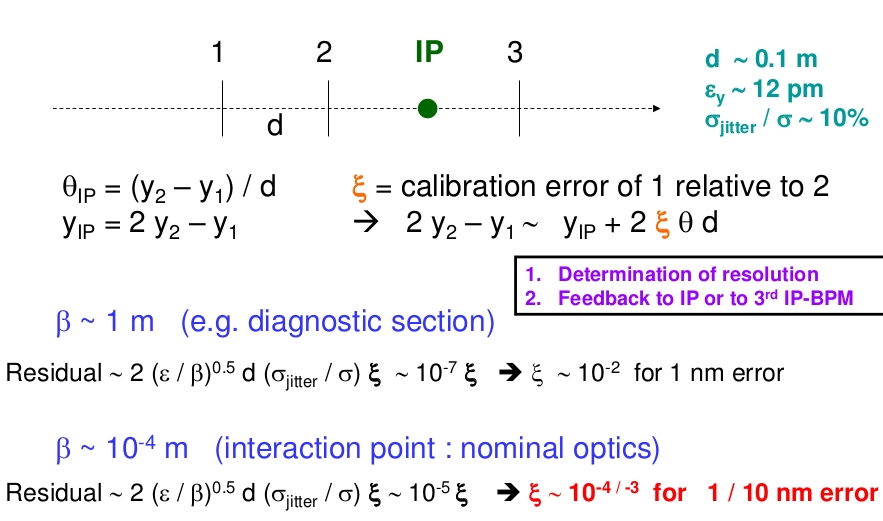
\includegraphics[angle=0,scale=0.35]{scalefactors.jpg}
{\LARGE
  \begin{itemize}
   \item Locate BPMs to enable the \textbf{ maximum possible} beam position resolution
   \item Precision $\sim 5\mu$m
   \item Calibration $\sim 10^{-4}$
  \end{itemize}
 \hspace*{5cm}$\Downarrow$\\
 Displace each BPM block \textbf{independently}
 }\par
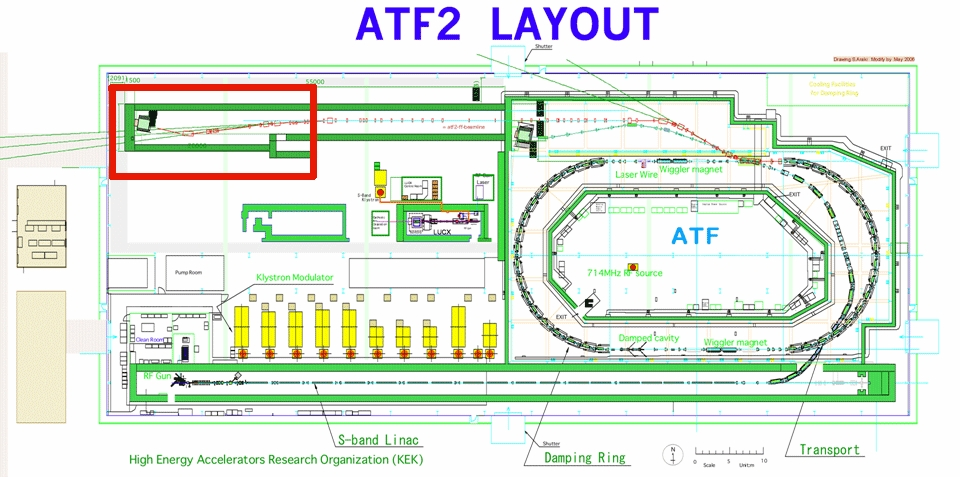
\includegraphics[angle=0,scale=0.2]{ATF2layout33.jpg}
% \end{frame}
% \begin{frame}
\hspace{1cm}
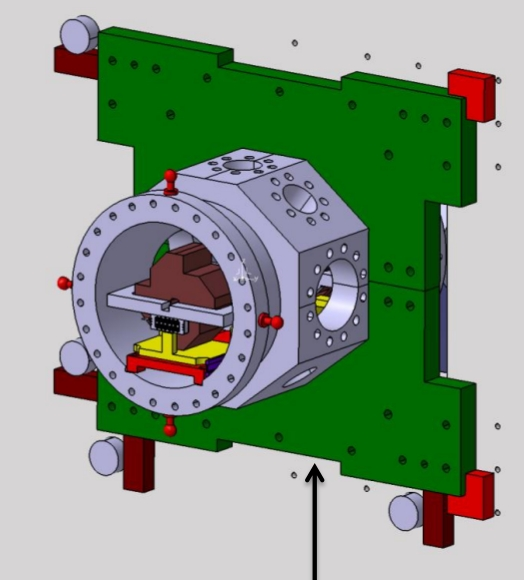
\includegraphics[angle=0,scale=0.16]{chambrevide.jpg}\\
\hspace*{1cm}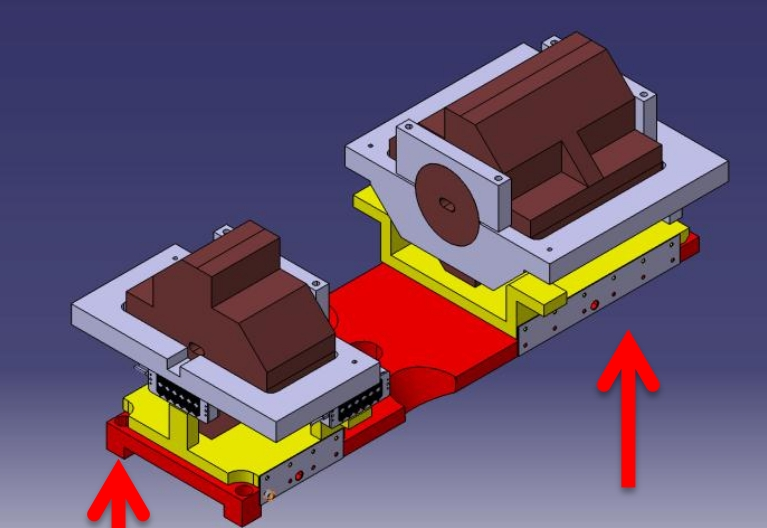
\includegraphics[angle=0,scale=0.22]{BPMs01.jpg}\hspace*{0.2cm}
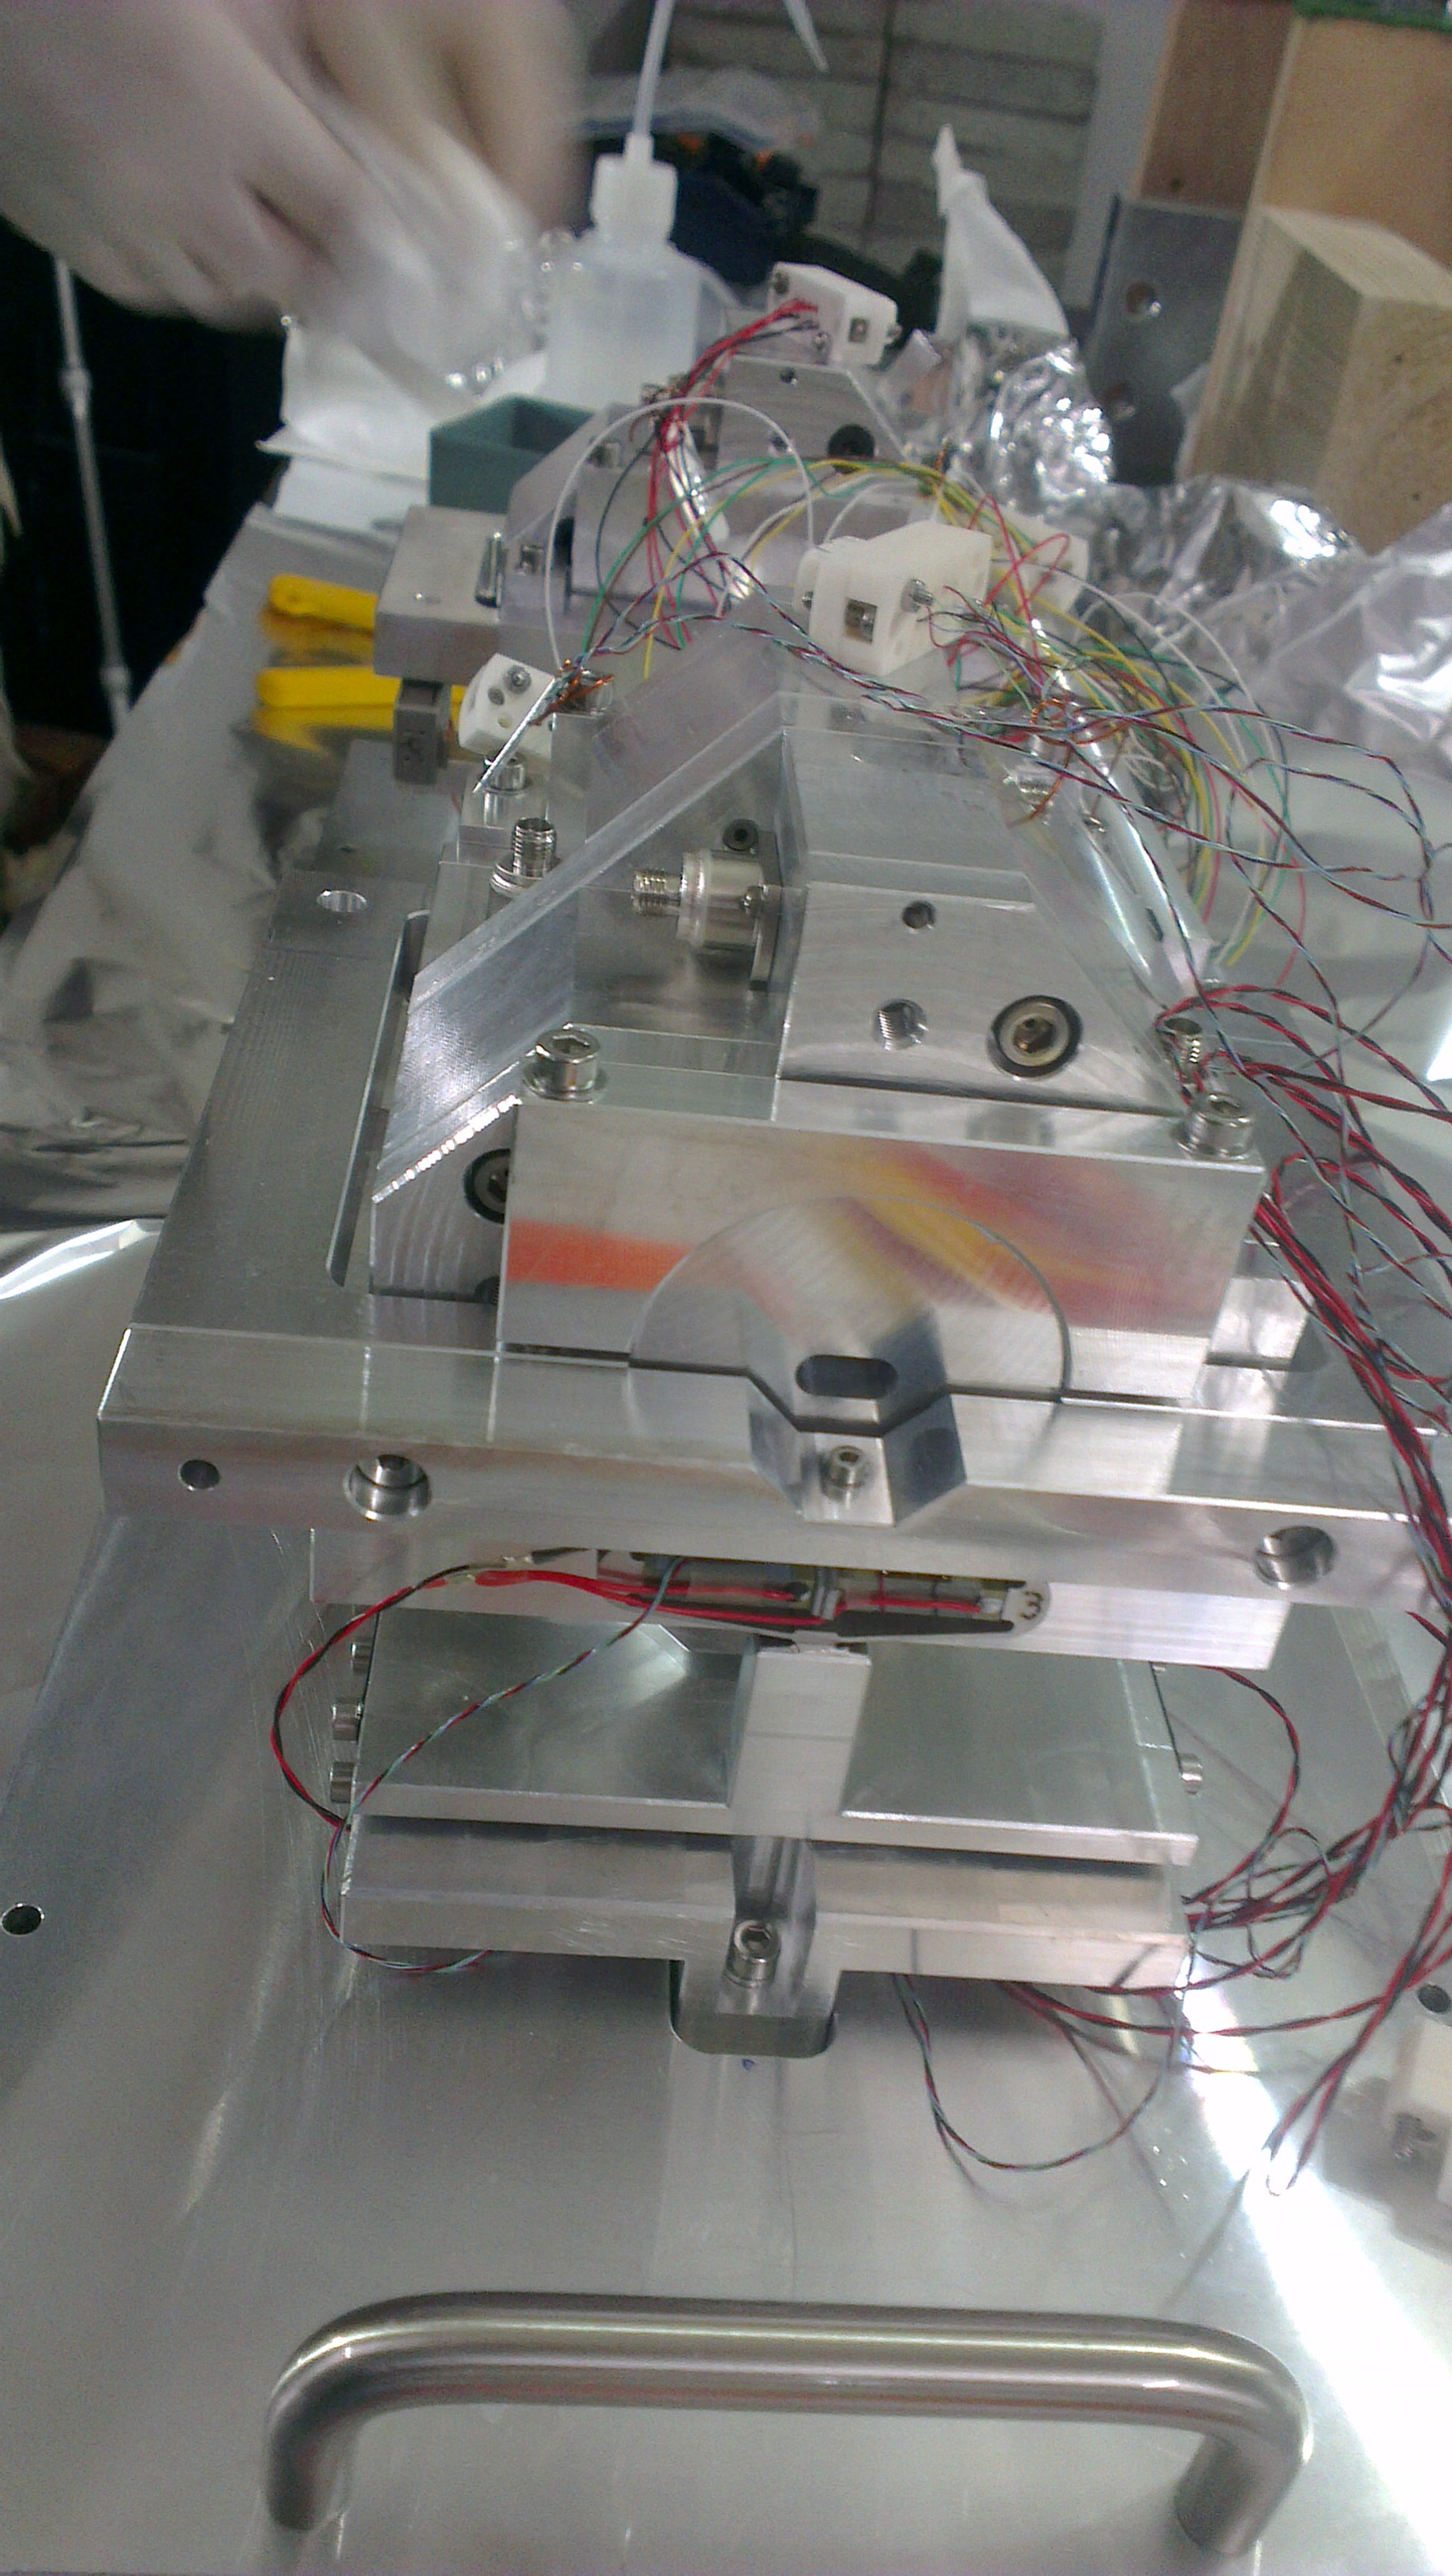
\includegraphics[angle=0,scale=0.0355]{IMAG0460.jpg}\par
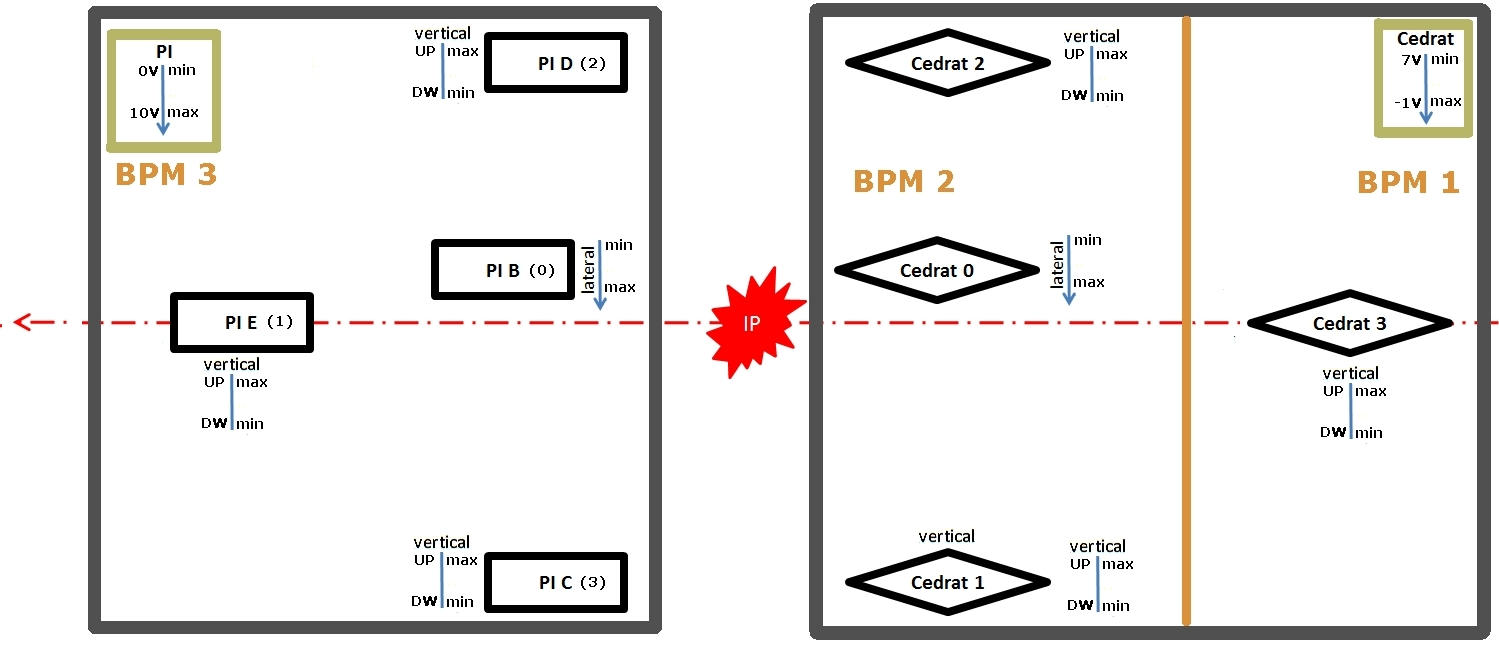
\includegraphics[angle=0,height=7.5cm,width=12cm]{interface.jpg}

\section{Alignment Requirements}
Considering the signal $S$ as the sum of the two outputs from the cavity (which are ideally 180$\deg$ separated).\par
\includegraphics[angle=0,scale=0.4]{electr2.jpg}\\
Signal $S$ for the vertical outputs of one BPM is composed of:
\begin{equation}
S = y_j+y+is_p(\theta_p+\theta_{pj})+s_{xy}[(x+x_j)+is_y(\theta_y+\theta_{yj})]+(x-x_j)\theta_r
\end{equation}
where $i$ is the imaginary number indicating a 90 degrees fase difference. $s_p$ is the sensitivity to angle, $s_{xy}$ is the inverse of X-Y isolation, $s_y$ is the yaw angle sensitivity. The sub-$j$ components are due to beam jitter and $x,y,\theta_p,\theta_r,\theta_y$, are the pitch, roll and yaw angles.

The objective is to measure $y_j$ with $10^{-4}$ or 1nm Precision. All other components are adding to error. All position errrors here are static, except the jitter components.

Using the nominal optics 1BX1BY, largest beam size is at BPMA, having 57.657$\mu$m beam size. Beam jitter will be considered 20\%, then $y_j$ is 11.531$\mu$m, or 10\%, then $y_j$ is 5.766$\mu$m.\par
In order to measure 1nm of 5.766um, it is necessary to use about 12.5 bits of discretisation ($2^{12.5}=5792$). On the other side as $1/10^{-4}$ is more than 1nm when 20\% jitter, then, we use 10 bits of discretisation ($2^{10}=1024$).\par
If we want to keep the same precision including tolerances, then total displacement (jitter + tolerances)/$2^{14}$ should be equal to either 1nm when 10\% jitter or $10^{-4}$ when 20\% jitter.
\begin{equation}
 (y_j+tolerances)/2^{14}=1\text{  nm, or, }\qquad (y_j+tolerances)/2^{14}=y_j/10^4
\end{equation}
We could separate the equation in real and imaginary components, where ideally, with perfect IQ rotation, all imaginary part can be substracted and the real part gives you information about position.\par
However, 


The acquisition system is 14 bits precision, then, only 1.5 bits are left for 10\% jitter and 4 bits for 10\% jitter.
